\section{Introduction}
Mixture-of-Experts (MoE) architectures~\cite{shazeer2017outrageously} are built on the observation that different inputs are best handled by different experts. Rather than passing every input through the full network, an MoE model routes each token to a small subset of feed-forward experts, so that total parameters can grow without a corresponding growth in per-token compute~\cite{fedus2022switch}. The mechanism that realizes this is the router: at each MoE layer, a small learned network produces a logit over the layer's experts for the current token, and the top-$k$ experts by logit are activated to process it. The router's logits thus determine, per token and per layer, which slice of the model's parameters participates in the forward pass, so that each input is processed by the experts best suited to handle it.

An analogous observation holds for safety. For a given input, different experts contribute differently not only to how well the model handles it, but also to how safely. On a risky query, some experts amplify unsafe behavior while others suppress it, and the split between the two depends on the query. This suggests that the same per-input routing mechanism that gives MoE its capability efficiency can also serve as the surface for alignment, with the router selecting experts based on safety relevance for each input.

A natural way to leverage this is to add a bias to the router that suppresses experts driving unsafe behavior and promotes those pulling toward refusal. As shown in Figure~\ref{fig:motivation}~(a), this turns the router itself into the surface on which alignment-enhancing intervention happens. Realizing this idea, however, raises two challenges.

\begin{figure}[t]
\centering
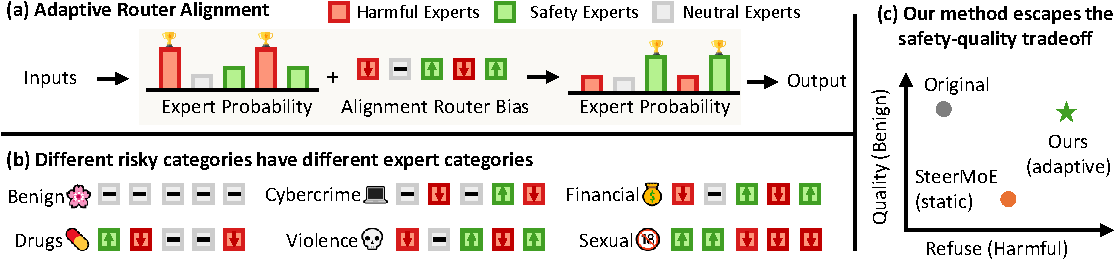
\includegraphics[width=\linewidth]{figures/motivation.pdf}
\caption{(a) \name: for each query, a per-query bias is added to the router logits to suppress experts driving unsafe behavior and promote those pulling toward refusal. (b) Different risk categories engage disjoint expert subsets. (c) \name escapes the safety-helpfulness trade-off incurred by the static design.}
\label{fig:motivation}
\end{figure}

The first challenge is \textbf{identification}. To compute an alignment router bias for a given query, we must know which experts are responsible for amplifying unsafe behavior on that query. A natural simplification is to assume the set of risk-amplifying experts is stable across harmful inputs and identify it once offline, as SteerMoE~\cite{fayyaz2025steermoe} does by contrasting expert activation rates between paired safe and unsafe responses to obtain a fixed pool that is then suppressed uniformly at inference. However, this stability assumption does not hold in practice. As shown in Figure~\ref{fig:motivation}~(b), harmful queries from different risk categories engage visibly disjoint expert subsets, each recruiting a different slice of the network. Specifically, across 200 risky inputs on OLMoE-1B-7B, the per-query top-$5$ most risk-amplifying experts overlap at pairwise Jaccard of only $0.11$. A pool identified once from aggregate statistics cannot match the expert structure that is actually risk-amplifying on a given query, suppressing experts that are irrelevant on this input while leaving the query's actual culprits untouched. Therefore, identification must instead be performed per query.

The second challenge is \textbf{modulation}. Even when the right experts are identified, the strength of the intervention should not be uniform across inputs. A clearly malicious prompt warrants a strong push toward refusal, an ambiguous prompt warrants less, and a benign prompt warrants none at all. The static design above takes a single fixed bias magnitude and applies it everywhere, which is mismatched to the distribution of inputs encountered at deployment. Tuned high enough to defend against the malicious prompt, it needlessly refuses benign queries. Tuned low enough to leave benign queries alone, it lets malicious prompts through.

Both challenges have visible consequences at deployment. Figure~\ref{fig:motivation}~(c) illustrates them simultaneously by plotting refusal rate on harmful prompts against quality on benign prompts. The static design~\citep{fayyaz2025steermoe} lands in the lower-left region. Identification fails per-query, refusing too few harmful inputs, and modulation fails per-query, refusing too many benign ones. An intervention that performs identification per query and modulates intervention strength per query escapes this trade-off, occupying the upper-right region where both axes improve together. Modulation, like identification, must be performed per query.

We propose \textbf{\name}, an alignment-enhancing technique inspired by MoE's per-input routing principle, addressing both challenges with a single forward-backward pass per input and no weight modification. It reads two signals from one shared probe of the input. For \textbf{identification}, the per-query risk-amplifying experts are exactly those whose router logits causally suppress the safety pathway on this specific input, and we localize them by computing the gradient $\partial s/\partial b$ of an output-safety score $s$ with respect to each router logit $b$, with the most-negative entries identifying the experts to suppress. For \textbf{modulation}, the intervention strength should track how harmful the query is rather than be set once for all queries, and we scale the alignment router bias by a harmfulness signal $\lambda(q)$ read from the same probe, so a clearly malicious prompt receives a strong push toward refusal and a benign prompt receives no intervention.

Extensive experiments demonstrate the effectiveness of our proposed method from multiple perspectives. Across three MoE backbones (OLMoE-1B-7B, Qwen1.5-MoE-A2.7B, and Mixtral-8x7B), \name{} improves average safety on six PandaGuard JBB risky-input families by $21.2$, $21.7$, and $23.0$ percentage points respectively, while preserving XSTest helpfulness within $0$\,pp of the unmodified backbone and MMLU within $0.3$\,pp. These results show that the same per-input routing mechanism that gives MoE its capability efficiency can be repurposed for alignment, lifting safety without sacrificing helpfulness.